\documentclass{article}

% Marges du papier
\usepackage[a4paper, margin=3cm, top=2cm]{geometry}
\usepackage[utf8]{inputenc}
\usepackage[frenchb]{babel}

% Pas d'indentation de chaque début de paragraphe
\setlength{\parindent}{0pt}
\usepackage{listings}
\usepackage{color}
\usepackage[toc,page]{appendix}
\usepackage{booktabs}
\usepackage{csquotes}
\usepackage{adjustbox}
\usepackage{tcolorbox}
\usepackage{tabularx}
\usepackage{graphicx}
\usepackage{url}

% Pour que les footnotes dans les tableaux fonctionnent \begin{savenotes} <tableau> \end{savenotes}
\usepackage{footnote}

\usepackage{pdflscape}
\usepackage{fancyhdr}
\usepackage[style=verbose,backend=bibtex]{biblatex}

% Path du dossier dans lequel se trouvent les images
\graphicspath{ {img/} }

% numéro de citation entre crochets. Ex: [3]
\renewcommand*{\thefootnote}{[\arabic{footnote}]}

% "Annexes" en français au lieu de "Appencies"
\renewcommand{\appendixtocname}{Annexes}
\renewcommand{\appendixpagename}{Annexes} 


\definecolor{codegreen}{rgb}{0,0.6,0}
\definecolor{codegray}{rgb}{0.5,0.5,0.5}
\definecolor{codepurple}{rgb}{0.58,0,0.82}
\definecolor{backcolour}{rgb}{0.95,0.95,0.92}

% Crée une boîte "importante" \begin{important}Ceci est important\end{important}t
\newenvironment{important}
    {
		\begin{tcolorbox}
		\begin{center}
		\includegraphics[scale=0.3]{important}
		\end{center}
		\par
    }
	{
		\end{tcolorbox}
	}

\definecolor{tableheader}{rgb}{0.95,0.95,0.92}
 
\lstdefinestyle{mystyle}{
    backgroundcolor=\color{backcolour},   
    commentstyle=\color{codegreen},
    keywordstyle=\color{blue},
    numberstyle=\tiny\color{codegray},
    stringstyle=\color{codepurple},
    basicstyle=\footnotesize,
    breakatwhitespace=false,         
    breaklines=true,                 
    captionpos=b,                    
    keepspaces=true,                 
    numbers=left,                    
    numbersep=5pt,                  
    showspaces=false,                
    showstringspaces=false,
    showtabs=false,                  
    tabsize=2
}

\lstset{%
	inputencoding=utf8,
	extendedchars=true,
	literate=%
	{é}{{\'{e}}}1
	{è}{{\`{e}}}1
	{ê}{{\^{e}}}1
	{ë}{{\¨{e}}}1
	{É}{{\'{E}}}1
	{Ê}{{\^{E}}}1
	{û}{{\^{u}}}1
	{ù}{{\`{u}}}1
	{â}{{\^{a}}}1
	{à}{{\`{a}}}1
	{á}{{\'{a}}}1
	{ã}{{\~{a}}}1
	{Á}{{\'{A}}}1
	{Â}{{\^{A}}}1
	{Ã}{{\~{A}}}1
	{ç}{{\c{c}}}1
	{Ç}{{\c{C}}}1
	{õ}{{\~{o}}}1
	{ó}{{\'{o}}}1
	{ô}{{\^{o}}}1
	{Õ}{{\~{O}}}1
	{Ó}{{\'{O}}}1
	{Ô}{{\^{O}}}1
	{î}{{\^{i}}}1
	{Î}{{\^{I}}}1
	{í}{{\'{i}}}1
	{Í}{{\~{Í}}}1
}

\lstdefinestyle{json}
{
  showstringspaces    = false,
  keywords            = {false,true},
  alsoletter          = 0123456789.,
  morestring          = [s]{"}{"},
  basicstyle          = \ttfamily,
  keywordstyle        = \ttfamily\bfseries,
}
 
\lstset{style=mystyle}

\usepackage{fancyhdr}
 
\pagestyle{fancy}
\fancyhf{}
% Header left
\fancyhead[RE,LO]{
\includegraphics[width=4cm]{heiglogo}}

% Header height
\setlength\headheight{1.5cm}

% Header right
\fancyhead[LE,RO]{WEBRAILS - Julien Amacher, Romain Maillard}

% Footer right
\fancyfoot[LE,RO]{\thepage}

\usepackage{xcolor,colortbl}

\bibliography{biblio} 


\selectlanguage{french}

\title{Projet WEBRAILS}
\date{2016}
\author{Julien Amacher, Romain Maillard}

\begin{document}


% Page de garde
\makeatletter         
\def\@maketitle{
\raggedright

\includegraphics[width=6cm]{heiglogo}\\[8ex]
\begin{center}
{\Huge \bfseries \sffamily \@title }\\[4ex]
{\Large  \@author}\\[6ex]
\@date\\[20ex]

{\large News}\\[8ex] 

\end{center}}
\makeatother


\maketitle
\thispagestyle{empty}
\newpage
\thispagestyle{empty}
\tableofcontents
\newpage

\section{Description}

Ce projet a pour but de réaliser une plate-forme permettant d'une part la rédaction de news et d'autre part leur consultation. Les rédacteurs écrivent et modifient des news, en y liant catégories (par ex: politique) et des sources (par ex: Paul Dupont). Chaque rédacteur travaille pour un média (par ex: France Info)

\section{Contraintes}

Les contraintes du projet sont les suivantes
\begin{itemize}
\item Le langage de programmation est Ruby on Rails (RoR)
\item La base de données est MySQL
\end{itemize}

\section{Cas d'utilisation}

Ce chapitre décrit les attentes et les fonctionnalités fournies pour chaque type de client de l’applicatif.

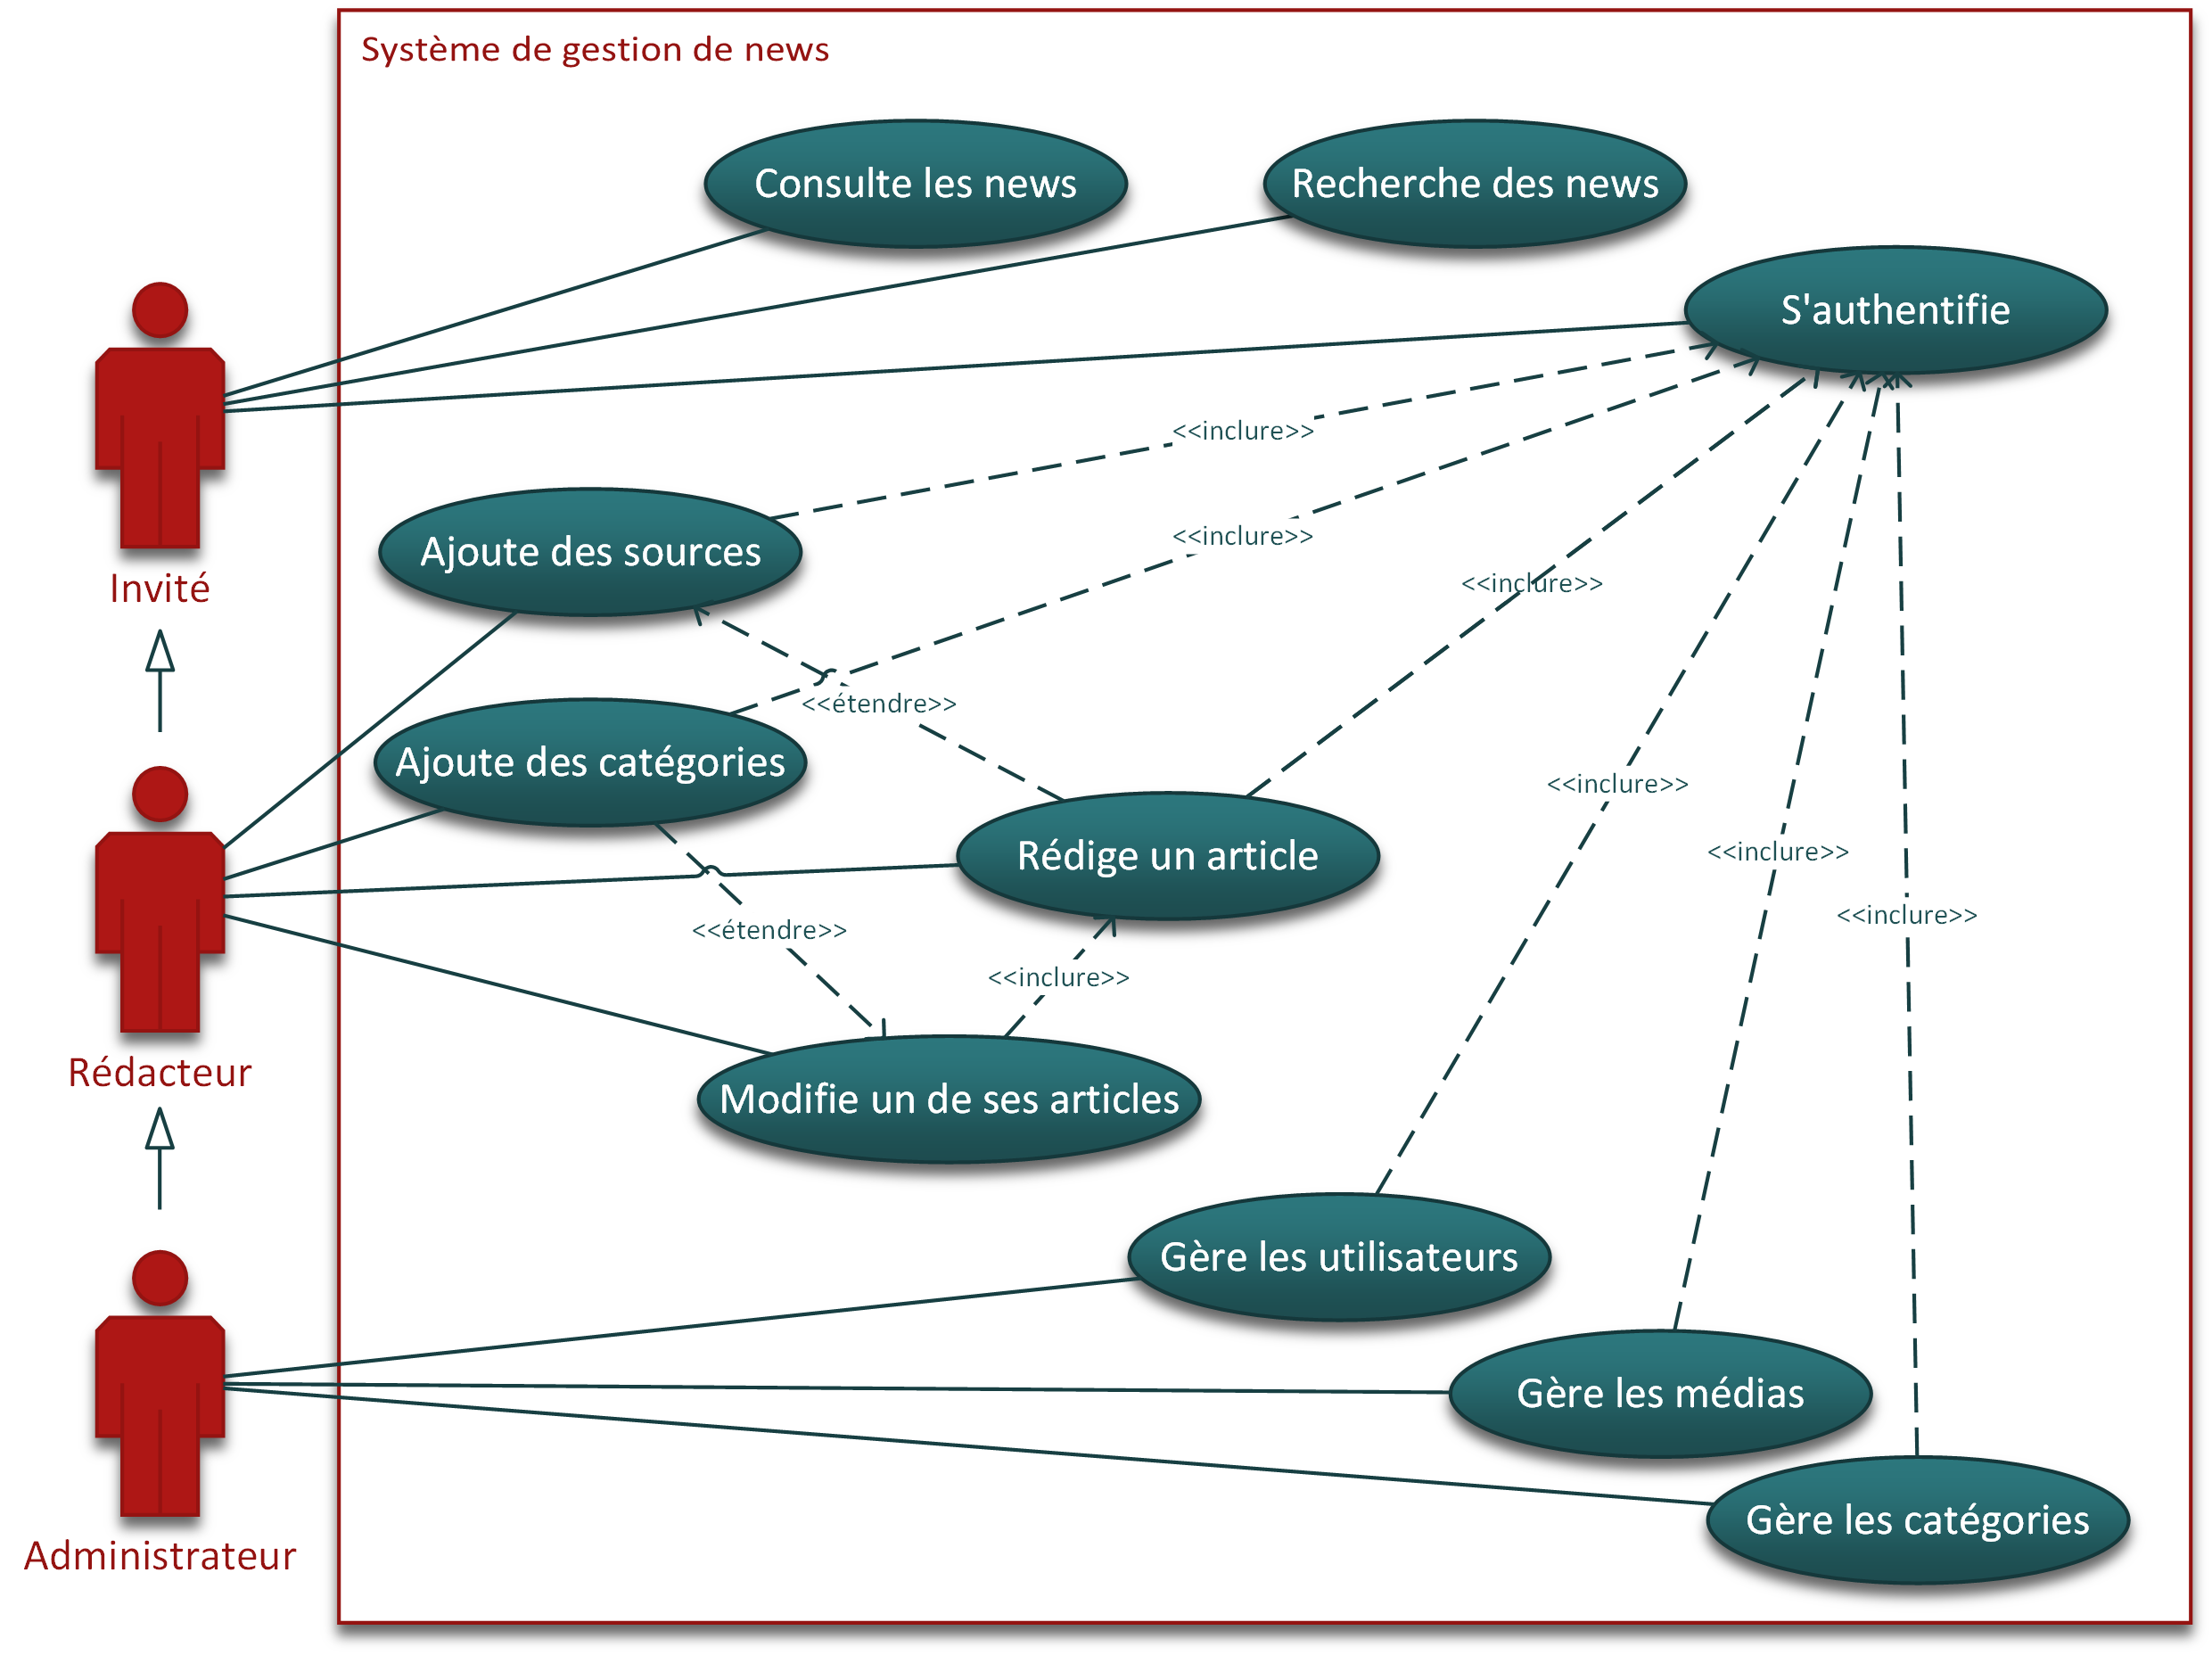
\includegraphics[width=\textwidth]{use_cases}


\subsection{Les invités}

\subsubsection{Consultent les news}

Ils peuvent librement consulter les news qu'ils désirent. Celles-ci sont présentes sur la page principale du site.

\subsubsection{S'authentifient}

Les invités s'authentifient en fournissant les informations suivantes :
\begin{itemize}
\item Leur adresse email
\item Leur mot de passe
\end{itemize}

Leur compte est ensuite identifié et leur rôle leur est attribué (rédacteur ou administrateur)

\subsubsection{Recherche des news}

Il est possible de rechercher une news par son titre, sa catégorie ou sa source.

\subsection{Les rédacteurs}

\subsubsection{Ajoutent une source à leur news}

Une news ayant au minimum une source, le rédacteur de la news peut en créer et en lier. Une news consiste en un titre, un chapeau ainsi qu'un contenu. 

\subsubsection{Ajoute une catégorie à leur news}

Une catégorie pouvant contenir plusieurs news (par exemple: politique), un rédacteur peut spécifier les catégories concernées par sa news.

\subsubsection{Rédige une news}

Le rédacteur peut écrire une news. Une news comprend un titre, un chapeau (extrait en gras), un contenu ainsi qu'une liste de sources et est contenue dans au moins une catégorie. U

Idéalement, les sources devraient pouvoir être créées `sur le vif` lors de la rédaction d'une news.

\subsubsection{Modifie une news}

Le rédacteur peut modifier une de ses news, cela inclut:
\begin{itemize}
\item Son titre
\item Son chapeau
\item Son contenu
\item Ses sources liées (en ajouter, en supprimer)
\item Ses catégories liées (en ajouter, en supprimer)
\end{itemize}

\subsection{Un administrateur}

\subsubsection{Gère les utilisateurs}

Un administrateur crée, modifie et supprime les comptes des utilisateurs du système.

\subsubsection{Gère les catégories}

Un administrateur gère les catégories : il peut en ajouter, modifier et supprimer.

\subsubsection{Gère les médias}

Un administrateur gère les médias : il peut en ajouter, modifier et supprimer. Chaque rédacteur est lié à un média et l'administrateur est le seul à pouvoir modifier à quel média le rédacteur est rattaché.

\newpage
\section{Base de données}

\subsubsection{MCD}

Le modèle conceptuel des données se présente comme suit:

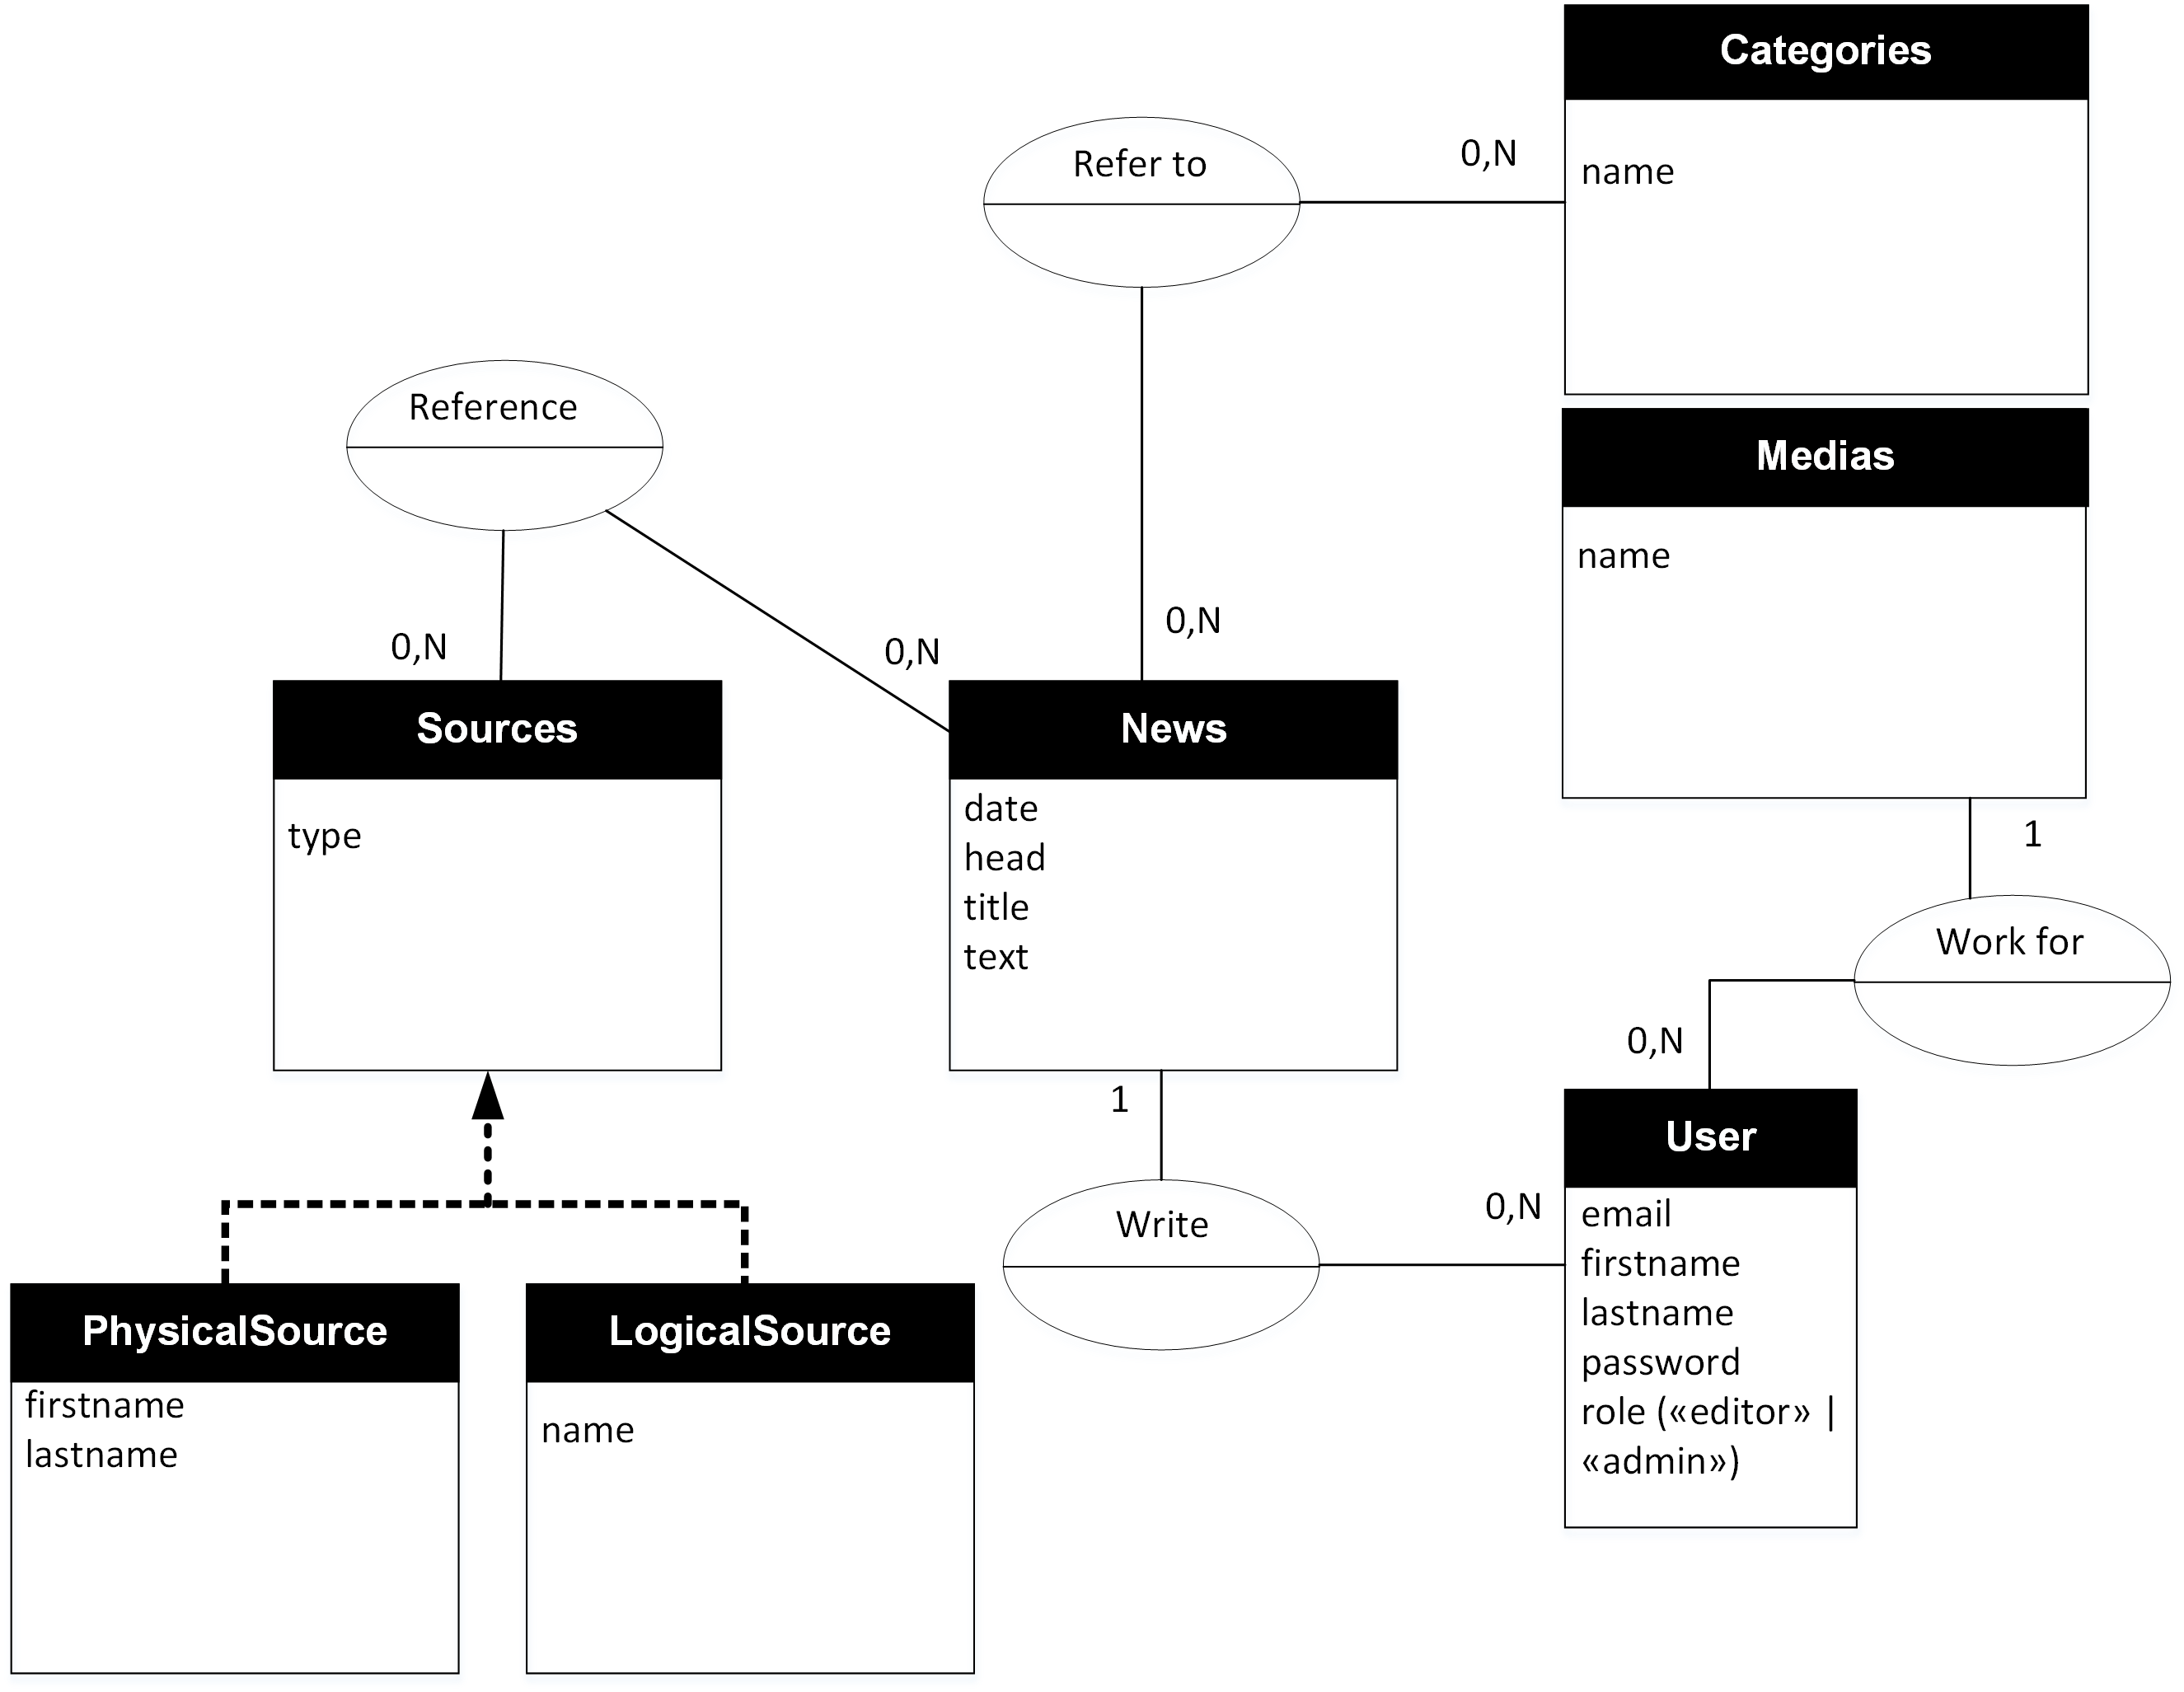
\includegraphics[width=\textwidth]{mcd}

Contraintes:
\begin{itemize}
\item Une news a au minimum une source liée
\item Une source fait référence à au minimum une catégorie (politique, économie, etc.)
\item Une source peut exister même si aucune news n'y fait référence, idem pour les catégories de news
\item Un rédacteur est lié à un média
\end{itemize}

\subsubsection{MPD}

\textbf{Users}

\begin{itemize}
\item firstname
\item lastname
\end{itemize}

Cancancan gère le rôle de l'utilisateur et Devise gère l'authentification (et y ajoute l'attribut email).

\textbf{Report}

\begin{itemize}
\item head
\item title
\item text
\end{itemize}

Chaque rapport a une date de création. Nous utilisons le champ created at de Rails.

\textbf{Sources}

\begin{itemize}
\item firstname
\item lastname
\item name
\item type
\end{itemize}

\textbf{Categories}

\begin{itemize}
\item name
\end{itemize}

\textbf{Medias}

\begin{itemize}
\item name
\end{itemize}

\section{Itérations}

\begin{itemize}
\item 3 mai
	\begin{itemize}
	\item Création de la base de données et des pages squelettes.
	\end{itemize}
	
\item 17 mai
	\begin{itemize}
	\item Ajout, modification et suppression de news, utilisateurs, catégories et médias fonctionnent.
	\end{itemize}

\item 7 juin
	\begin{itemize}
	\item Fonctionnalité de recherche terminée + droits d'accès implémentés.
	\end{itemize}
\end{itemize}

\section{Fonctionnalités Ajax}

La recherche des news se fait via Ajax. La recherche se fait par news, catégorie et source. Le contenu, titre et chapeau de la news sont considérés lors de la recherche.

\printbibliography

%\newpage
%\begin{appendices}

%\newpage
%\section{Annexe 1}
%\newpage
%\section{Annexe 2}
%\end{appendices}

\end{document}